\begin{frame}
\frametitle{Android + Akka + Spray.io}

\begin{columns}[c]
	\begin{column}[t]{.45\textwidth}
		\vskip-6em
		\begin{enumerate}
			\item Scala na Androidzie --- można?
			\only<2->{\item Serwer(y): Akka + Spray.io.
				\item Telefon --- aktor (\emph{stateless!}).}
			\only<3->{\item Push? REST Spray.io z long-pollingiem.
				\item To samo API dla webapp.}
		\end{enumerate}
	\end{column}
	\begin{column}{.45\textwidth}
		\begin{figure}
			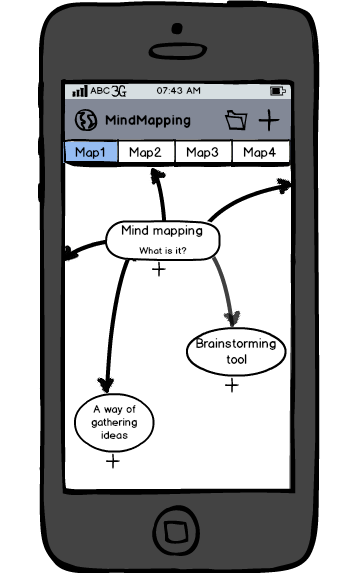
\includegraphics[height=6cm]{graphics-mockup-map}
		\end{figure}
	\end{column}
\end{columns}

\end{frame}
